




\section{Time to connect socket (ANOVA)}
\label{app:anova_socket}

%%%%%%%%%%%%%%%%%%%%%%%%%%%%%%%%%%%%%%%%%%%%%%%%%%%%%%%%%%%%%%%%%%%%%%%%%%%%%%%%%%%%%%%%%%%%%
%--------------------------------------- Jing begin ---------------------------------------

We aim to test if there is any significant difference in time taken to connect socket A and B. We hypothesised that socket A requires longer time than socket B. 


We have collected 10 subjects and spited them equally into two groups. All subjects were trained to plug the two sockets before the experiments and each of them repeated both sockets two times. The sequences of plugging the two sockets for the two groups are the opposite. Group 1 started with socket A then socket B, while group 2 reversed the order (figure \ref{figuretimesubject}). 


Before applying statistical test to compare the time used of the two groups, we tested the normality of the distributions of time used for the two sockets from the two groups. We applied Shapiro-Wilk test of normality in R and used Q-Q plot to compare the shapes of distributions (figure \ref{QQplot}). None of the distributions of time taken by the two groups and two sockets are normal (p< 0.0001,Shapiro-Wilk test). Therefore, we chose a non-parametric test to compare the distributions of time between different sockets. Since socket A and B were performed by related samples, we applied paired difference test, Wilcoxon signed-rank test, to assess whether their population mean ranks differ. Socket A took significantly longer time than socket B and this result was observed in the two groups (group 1 p<0.0001, group 2 p=0.0002,Wilcoxon signed-rank test, figure \ref{figuretimesubgroup}).   

%--------------------------------------- Jing end ---------------------------------------


% \begin{enumerate}
%  \item $H_o$: There is no difference in the time taken to connect Socket A or B. (check whether both 
%  sockets have the same difficulty).
%  \item $H_o$: There is no improvement between the first and second search.
%  \item $H_o$:
% \end{enumerate}

\begin{figure}
 \centering
 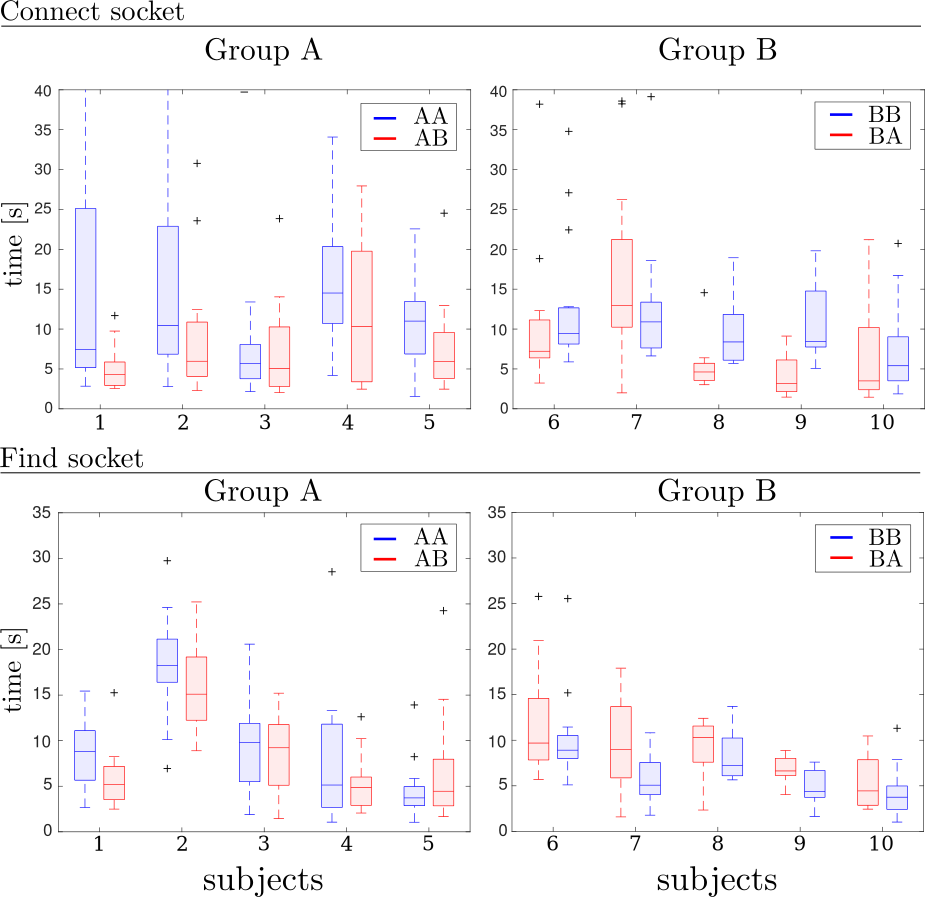
\includegraphics[width=\textwidth]{./ch4-PiH/Figures/time_taken_subgroup.pdf}
 \caption{Time taken to find and connect the plug to the power socket. \textbf{Top:} 
 Time taken to connect the plug to the socket once the socket is localised. For most subjects the median value of the taken time is higher 
 for socket A when compared with socket B. \textbf{Bottom}: time taken to localise the socket. For the second
 search, AB and BA, it seams that the subjects are faster indicating learning during the experiment.
 }
 \label{figuretimesubject}
\end{figure}

\begin{figure}
   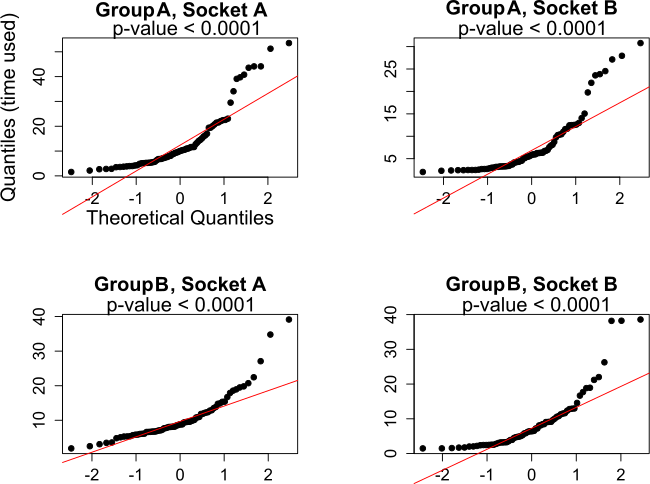
\includegraphics[width=0.8\textwidth]{./ch4-PiH/Figures/QQplot.pdf}
   \caption{QQ plot of time taken for two sockets by two groups. \textbf{Top left}: group 1 for socket A;\textbf{Top right}: group 1 for socket B;\textbf{Bottom left}: group 2 for socket A;\textbf{Bottom right}: group 2 for socket B. The p-values above plots are from Shapiro-Wilk test.}
   \label{QQplot}
\end{figure}


\begin{figure}
  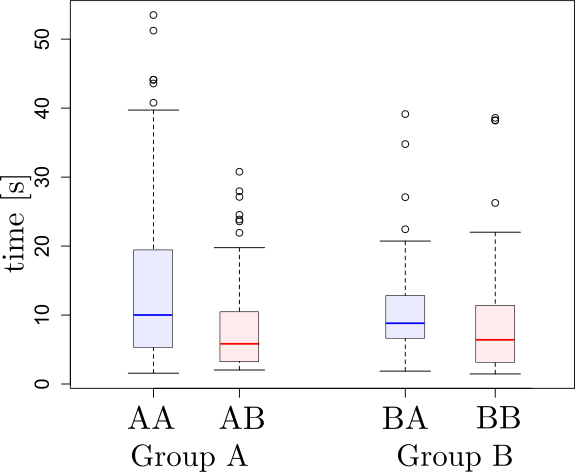
\includegraphics[width=0.8\textwidth]{./ch4-PiH/Figures/Group_Socket.pdf}
   \caption{Box plot of time taken for two sockets by two groups. \textbf{Left}: times of group 1 subjects took to perform socket A and B;\textbf{Right}: times of group 2 subjects took to perform socket B and A. }
   \label{figuretimesubgroup}
\end{figure}

% % 1) Is there are a difference across groups 
% % 2) Is there a difference between the two sockets
% The null hypothesis is that there is no difference in the time taken to connect socket A or B. The result of the one-way anova
% is given in Table \ref{tab:ch4:anova_socket}. The null hypothesis is rejected at high significant level (***) indicating that 
% there is a difference between the sockets. According to the linear model it takes on average 4 seconds less to connect socket B 
% than it does for socket A.
  
% \begin{table}[h]
% \centering
% \begin{tabular}{lcc}
%   \hline
%           &   F    & Pr(>F)  	     \\ \hline
%    socket & 13.9   &  0.000232 *** 
% \end{tabular}
% \caption{One way anova of the time taken to connect two sockets A and B. There is a significant difference.}
% \label{tab:ch4:anova_socket}
% \end{table}
% 
% We tested whether the group order had an effect on the connection time. We fitted a linear model
% with the predictor being time and the factors being the group (One or Two), the socket type (A or B) 
% and the subject's ID (1 to 10):
% \begin{equation}
%  time = \beta_0 + \beta_1\, group + \beta_2\, socket + \beta_3\, subject
% \end{equation}
% and did the corresponding anova analysis on this linear model. We found that the difference between the sockets 
% remained significant.

 

